RRTs are able to find a trajectory connecting two states: a starting one $x_o$ and an ending one $x_f$ building a search tree $T(x_o)$.
Each node $x_i \in T$ (apart from the root) is connected to its unique father $x_{fi}$ by a trajectory $\tau_{fi \rightarrow i}$. In the following of this article, we will use also this notation: $Fath(x_i)=x_{fi}$.
%The root $x_o$ is the only node not having a father ($Fath(x_o)=\emptyset$). 
The set $\mathcal{X} \subseteq \mathbb{R}^{d} $ will contain all the possible states $x$, while $\underline{\mathcal{X}} \subseteq \mathcal{X}$ is a subset describing the admissible region induced by a series of constraints to be considered. 
%If we consider a pure robotic path planning problem, they are represented by the presence of obstacles populating the workspace of the robot, that make some state (i.e. pose for the robot) not feasible. However, according to nature of the problem considered, they can assume also different meanings (see the examples in Sections \ref{sec:probl_A}, \ref{sec:probl_A} and \ref{sec:probl_C}).
The basic version of an RRT algorithm is described by Algorithm \ref{alg:RRT_single} (due to space limitations, the Steer procedure is not detailed, even though its behaviour it's heuristically explained below).

\begin{algorithm}
\caption{Canonical RRT}\label{alg:RRT_single}
\begin{algorithmic}[1]
\Procedure{RRT search}{$x_o$, $x_f$} 
\State $T(x_o)= \lbrace x_o \rbrace$; 
\For{\texttt{k=1:$I$}}
	\State \texttt{sample a}\,\,\, $x_R \in  \mathcal{X}$; 
	\State $x_s$ = Expand($T , x_R$);
	\If{\texttt{$x_s \in \underline{\mathcal{X}}$} AND \texttt{$\Vert x_s - x_f \Vert \leq \epsilon$}}
		\State \Return Path to root($x_s$)$ \cup x_f$;	
	\EndIf
\EndFor
\EndProcedure
\\
\Procedure{Expand}{$T, x_R$}
\State $x_{Nearest}=$Nearest Neighbour($T, x_R$) ;
\State $x_s=$ Steer($T, x_{Nearest}, x_R$);
\If{\texttt{$x_s \in \underline{\mathcal{X}}$}}
\State $Fath(x_s)=x_{Nearest}$;
\State $T = T \cup x_s$;
\EndIf
\Return $x_s$;
\EndProcedure
\\
\Procedure{Nearest Neighbour}{$T, x_R$}
\State \Return $\underset{x_i \in T}{\operatorname{argmin}}( C(\tau_{i \rightarrow R } ) )$;
\EndProcedure
\end{algorithmic}
\end{algorithm}

The Steer function in the $Expand$ procedure is problem-dependent. Basically, It has the aim to extend a certain state $x_i$ already inserted in the searching tree, toward another one $x_R$. For this purpose, an optimal trajectory $\tau_{ i \rightarrow R}$, agnostic of the constraints, going from $x_i$ to $x_R$ is taken into account. A series of equispaced states $x^{1,\cdots,K}_s$ lying along $\tau$, are verified to be in $\underline{X}$, in order to find the furthest one from $x_i$ (denoted as $x_s$) admitted by constraints. When none of the states $x^{1,\cdots,K}_s$ result to be in $\underline{X}$, the first intermediate state computed is returned, even though it is considered not valid, refer also to Figure \ref{fig:Steer}.
\begin{figure}
	\centering
\def\svgwidth{0.8 \textwidth}
\import{Immagini/pdf/}{Steer.pdf_tex} 
	\caption{The dashed curves in both pictures are the optimal trajectories connecting the pair of states $x_{Nearest}$,$x_{target}$, while the filled areas are regions of $X$ not allowed by constraints.	
	The steering procedure integrates with a fixed step the optimal trajectory, with the aim of finding the furthest admissible state from $x_{Nearest}$ lying along the trajectory. For the example on the right, the steering is not possible: the first state obtained is returned as $x_s$ although is not valid.}
	\label{fig:Steer}
\end{figure} 



% \footnote{Notice that in the general case, it is not guaranteed that $C(\tau_{ 1 \rightarrow 2}) = C(\tau_{ 2 \rightarrow 1})$}. 
The Nearest Neighbour procedure relies on the definition of a cost function $C(\tau)$. Therefore, the closeness of states does not take into account the shape of $\underline{\mathcal{X}}$.
The algorithm terminates when a steered configuration $x_s$ sufficiently close to $x_f$ is found.     
\\
\\
The previously described algorithm can be modified to consider a bidirectional strategy, expanding simultaneously two different trees \cite{RRT_bid} (see the picture in the middle of Figure \ref{fig:Tree_Comparison}). Indeed, at every iteration one of the two trees is extended toward a random state. Then, the other tree is extended toward the steered state previously obtained. At the next iteration, the roles of the trees are inverted. The algorithm stops, when the two trees meet each other. The detailed pseudocode is reported by Algorithm \ref{alg:RRT_bid}.

\begin{algorithm}
\caption{Bidirectional RRT}\label{alg:RRT_bid}
\begin{algorithmic}[1]
\Procedure{RRT bidirectional search}{$x_o$, $x_f$} 
\State $T_{master}= T(x_o)= \lbrace x_o \rbrace$;  
\State $T_{slave} = T(x_f)= \lbrace x_f \rbrace$; 
\For{\texttt{k=1:$\frac{I}{2}$}}
	\State \texttt{sample a}\,\,\, $x_R \in  \mathcal{X}$; 
	\State $x_s =$ Expand($T_{master} , x_R$) ;
	\If{\texttt{$x_s \in \underline{X}$} }
		\State $x_{s2} =$ Expand($T_{slave} , x_s$) ;
		\If{\texttt{$x_{s2} \in \underline{X}$} AND \texttt{$\Vert x_s - x_{s2} \Vert \leq \epsilon$}}
		\State $Path_1=$Path to root($x_s$);
		\State $Path_2=$Revert(Path to root($x_{s2}$));
		\State \Return $Path_1 \cup Path_2$;
		\EndIf
	\EndIf
	\State Swap($T_{master}$, $T_{slave}$);
\EndFor
\EndProcedure
\end{algorithmic}
\end{algorithm}

This solution offers several advantages. For instance, the computational times absorbed by the Nearest Neighbour search is reduced since this operation is done separately for the two trees and each tree contains at an average half of the states computed (see Section \ref{Sec:cmpt_time_serial}).
\\
\\
Notice that there are many (possibly infinite) $\tau_{o \rightarrow f} \subset \underline{ \mathcal{X} }$. Among the aforementioned set, we might be interested in finding the trajectory minimizing $C(\tau_{o \rightarrow f})$. 
The basic version of the RRT algorithm is proved to find with a probability equal to 1, a suboptimal solution \cite{RRT_star}.
The optimality issue is addressed by a variant of the RRT, called RRT* \cite{RRT_star}, whose pseudocode is contained in Algorithm \ref{alg:RRT_star} ($d$ is the cardinality of $\mathcal{X}$).
Essentially, the RRT* version, after inserting in the search tree a newer steered state, tries to undertake local improvements to the connectivity of the tree, in order to minimize the cost-to-go of the states in the $Near$ set. This is proved to converge to the optimal solution. 
There are no precise stopping criteria for the RRT*.
\\
Figure \ref{fig:Tree_Comparison} reports some examples of trees obtained by following the three exposed strategies on the use-case detailed in Section \ref{sec:probl_1}.

%\\
%Figure \ref{fig:Extend} summarizes the computation steps involved in the tree expansion, while 
%Figure \ref{fig:Tree_Comparison} reports some examples of trees obtained by following the three exposed strategies on the use-case detailed in Section \ref{sec:probl_1}.

\begin{algorithm}
\caption{RRT*}\label{alg:RRT_star}
\begin{algorithmic}[1]
\Procedure{RRT* search}{$x_o$, $x_f$} 
\State $T(x_o)=\lbrace x_o \rbrace$; 
\State $Sol=\emptyset$;
\For{\texttt{k=1:$I$}}
	\State \texttt{sample a}\,\,\, $x_R \in  \mathcal{X}$; 
	\State $x_s =$Expand star($T , x_R$);
	\If{\texttt{$x_s \in \underline{\mathcal{X}}$} AND \texttt{$\Vert x_s - x_f \Vert \leq \epsilon$}}
		\State $Sol= Sol \cup x_s$;
	\EndIf
\EndFor
\State $x_{best} = \underset{x_S \in Sol}{\operatorname{argmin}}$( Cost to root($x_S$) );
\State \Return Path to root$(x_{best}) \cup x_f$;
\EndProcedure
\\
\Procedure{Expand star}{$T,x_R$}
\State $x_s$=Expand($T,x_R$);
\State $N=size(T)$;
\State $Near=\lbrace x_i \in T | C(\tau_{i \rightarrow s}) <= \gamma {(\frac{log(N)}{N})}^{\frac{1}{d}}  \rbrace$;
\State Rewird($Near,x_s$);
\State \Return $x_s$;
\EndProcedure
\\
\Procedure{Rewird}{$Near,x_s$}
\State $x_{best fath} = x_{Nearest}$, $C_{min} = C(\tau_{Nearest \rightarrow s})$;
\For{\texttt{$x_n \in Near$}}
\If{\texttt{$\tau_{n \rightarrow s} \subset \underline{\mathcal{X}}$} AND \texttt{$C(\tau_{n \rightarrow s}) < C_{min}$}}
\State $C_{min}=C(\tau_{n \rightarrow s})$; $x_{best fath}=x_n$;
\EndIf
\EndFor
\State $Fath(x_s)=x_{best fath}$;
\State $C_s=$Cost to root($x_s$); 
\For{\texttt{$x_n \in Near$}}
\If{\texttt{$\tau_{s \rightarrow n} \subset \underline{\mathcal{X}}$}}
	\State $C_n=C(\tau_{s \rightarrow n}) + C_s$
\If{\texttt{$C_n <$ Cost to root($x_n$)}}
	\State $Fath(x_n)=x_s$;
\EndIf
\EndIf
\EndFor
\EndProcedure
\\
\Procedure{Cost to root}{$x_i$}
\State \Return $\sum_{x_p \in Path to root(x_i)} C(\tau_{Fath(p) \rightarrow p})$;
\EndProcedure
\end{algorithmic}
\end{algorithm}



%\begin{figure}
%	\centering
%\subfloat[]{\includegraphics[width=0.5\textwidth]{Immagini/pdf/Expand.pdf} \label{fig:Extend_01}}
%\caption{Steps involved for extending the search tree(s). 
%Those operations that require to scan every element contained in the search tree are shaded with a red color.}
%	\label{fig:Extend}
%\end{figure}
   
%\begin{figure}
%	\centering
%\subfloat[]{\includegraphics[width=0.5\textwidth]{Immagini/pdf/Expand.pdf} \label{fig:Extend_01}}\\
%\subfloat[]{\includegraphics[width=0.5\textwidth]{Immagini/pdf/Expand_bid.pdf} \label{fig:Extend_02}}
%\caption{Steps involved for extending the search tree(s). On the top: considering the basilar version of RRT and the RRT* one; on the bottom the bidirectional formulation. 
%In the top picture, those operations that require to scan every element contained in the search tree are shaded with a red color.}
%	\label{fig:Extend}
%\end{figure}

\subsection{Computational time analysis} \label{Sec:cmpt_time_serial}

Let $t_{\tau}$ denotes the mean time absorbed by the computation of an optimal trajectory $\tau$ connecting two states and $t_{V}$ the mean time required to check whether a certain state $x$ is contained within $\underline{X}$. The proportion between the two aforementioned quantities can vary a lot, considering the specific planning problem addressed.  
The total computation time $T$ absorbed by the invocation of a basic RRT algorithm can be estimated as follows:
\begin{eqnarray}
T &=& T_{\tau} + T_V \nonumber\\
T_{\tau} & = & \mathcal{O} \left( \sum_{i=1}^I ((i+1)t_{\tau}) \right) = \mathcal{O} \left( \frac{I(I+1)}{2} t_{\tau} \right) \nonumber\\
T_{V} & = & \mathcal{O} \left( I t_V \right) 
\label{eq:T_serial_single}
\end{eqnarray}
where $I$ is the number of iterations needed to complete the search. 
Indeed, at every iteration $i$, in the worst case, the tree contains $i$ elements for which the nearest neighbour search absorbs $i$ evaluations of $\tau$; while every expansion of the tree requires at least one feasibility check. Actually, at most $m$ checks are needed, where $m$ is the maximal number of extensions considered by the steering process (Figure \ref{fig:Steer}). However, this detail does not alter the fact that $T_V$ grows linearly with $I$. 
\\
When considering the bidirectional version, assuming the same value for $I$, we have roughly half of the nodes in every tree and therefore the time spent for the Nearest Neighbour search changes, leading to:
\begin{eqnarray}
T_{\tau} = \mathcal{O} \left( \frac{I(I+1)}{4} t_{\tau} \right)
\label{eq:T_serial_bid}
\end{eqnarray}
Finally, when considering the RRT* formulation, the Near set determination and the evaluation of the possible reconnection (also called rewirds) drastically improves the computational time $T$, leading to:
\begin{eqnarray}
T &=& T_{\tau} + T_V \nonumber + T_{Rew}\\
T_{\tau} &= & \mathcal{O} \left(  I(I+1) t_{\tau} \right) \nonumber\\ 
T_{Rew} &= & \mathcal{O} \left( \gamma t_V \sum_{i=1}^I \left( \frac{log(i)}{i}^{\frac{1}{d}} \right)  \right)
  \label{eq:T_serial_star}
\end{eqnarray}
%assuming the same $T_V$ of equation \ref{eq:T_serial_single}.

\begin{figure}
	\centering
	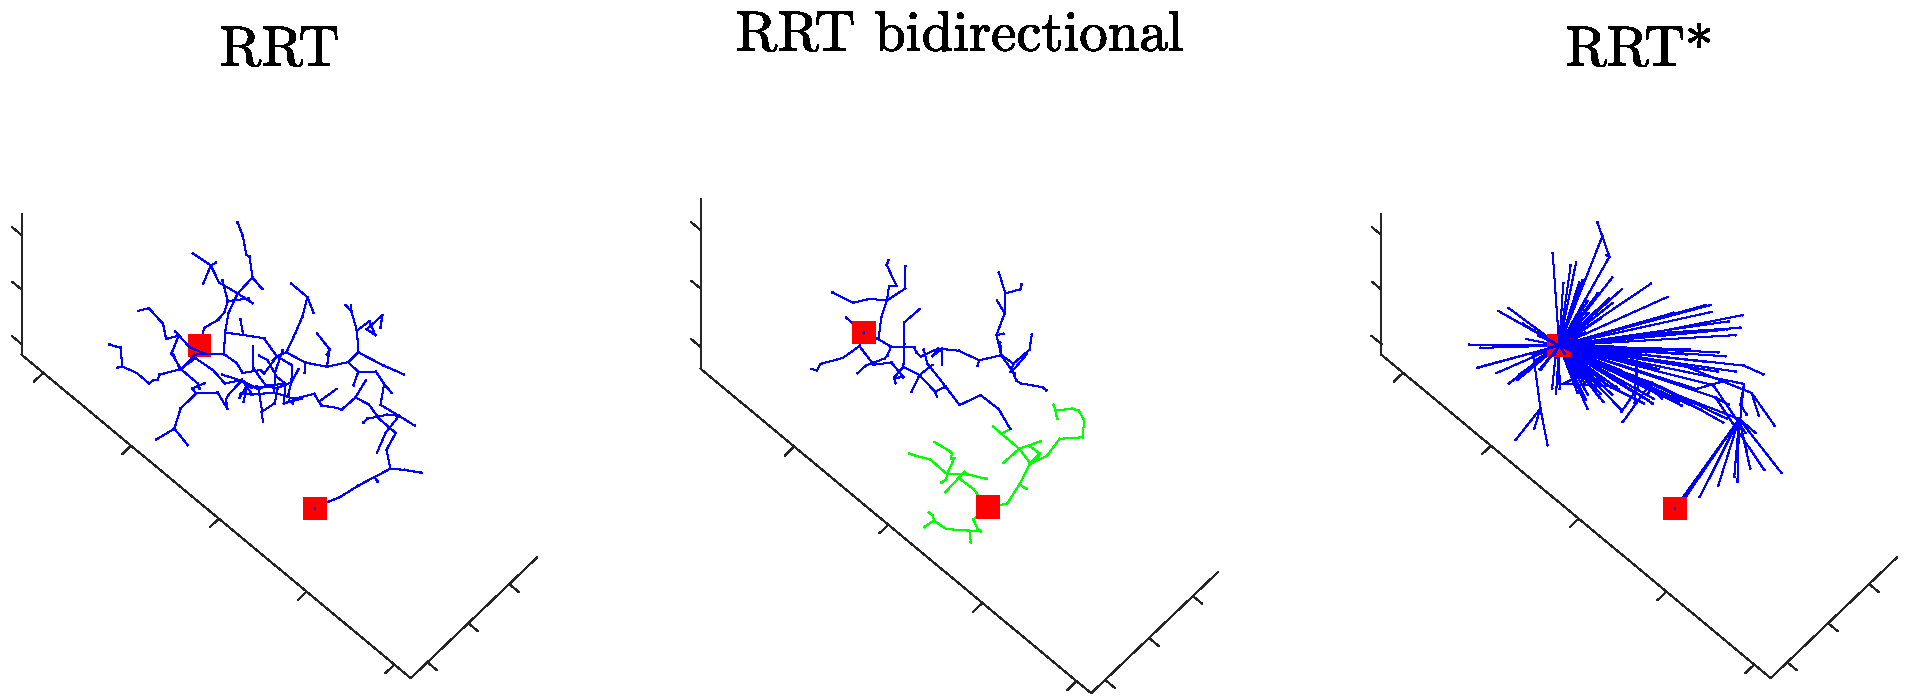
\includegraphics[width=0.5\textwidth]{Immagini/pdf/Tree_comparison_Chiara.pdf}
\caption{Examples of trees obtained when solving the planning problem detailed in Section \ref{sec:probl_1}. In all the pictures the states $x_o$ and $x_f$ are depicted as big red squares. 
%The nodes in the tree resulting by applying the RRT* have a reduced cost to go 
%( trajectories  connecting the states are simple segments in the joint space, whose cost is assumed to be the length of such a segment). 
 }
	\label{fig:Tree_Comparison}
\end{figure}